\chapter{Development support} 
\label{ch:Chapter4}
\vfill \minitoc \newpage

\section{Azure DevOps Services}

To ease development the group decided to use \textit{\cite{azuredevops}}. This platform provides development collaboration tools along with mechanisms that allow for a better work environment that follow DevOps practices.

Figure~\ref{fig:DevopsTasks1} illustrates DevOps Work Items (Azure Boards).

From the many tools provided by the service, the following are the ones used in this project:
\begin{itemize}
	\item Azure Boards
	\item Azure Repos
	\item Azure Pipelines
	\item Azure Artifacts
\end{itemize}


\begin{figure}[!ht]
	\centering
	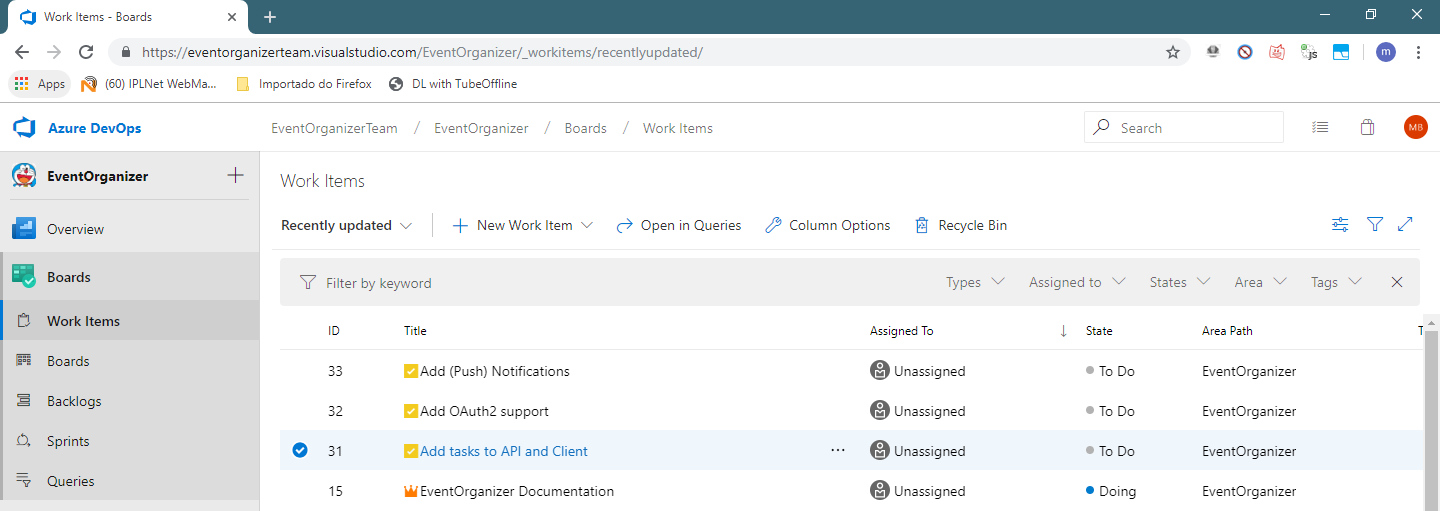
\includegraphics[width=0.75\textwidth]{./Chapter4/Figures/DevopsTasks1.png}
	\caption{DevOps Boards Work Items}
	\label{fig:DevopsTasks1}
\end{figure}

\subsection{Azure Repos}
Azure Repos is a set of version control tools, allowing for multiple repositories, each one having its own version control system. For this project four repositories where created:

\begin{itemize}
	\item EventOrganizer.WebApi – Where the source code for the EventAPI and its HTTP Client is maintained.
	\item EventOrganizer.Client – Where the Xamarin client application source code is maintained.
	\item EventOrganizer.Database – Repository containing the scripts and backups for database management.
	\item EventOrganizer.Documentation – Dedicated to gather project documentation used in development.
	\item EventOrganizer.MusicApi – Contains the source code for the Music Web Api and its HTTP Client.
\end{itemize}

Figure~\ref{fig:BranchingStrategy} illustrates the feature branching strategy used.

Wanting to keep the development repositories, EventOrganizer.WebApi, EventOrganizer.MusicApi and EventOrganizer.Client organized and easy to maintain, the group decided to use the following branching strategy:

\begin{figure}[!ht]
	\centering
	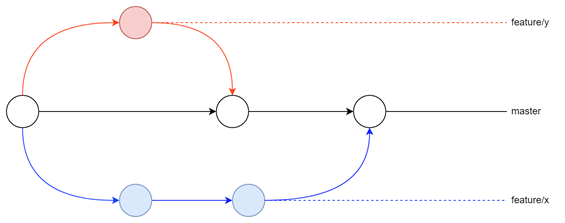
\includegraphics[width=0.75\textwidth]{./Chapter4/Figures/BranchingStrategy.png}
	\caption{Feature Branching Strategy}
	\label{fig:BranchingStrategy}
\end{figure}

This branching strategy consists of creating a feature branch for each new functionality that needs to be implemented. This, combined with frequent pull requests, helped the team maintaining the source code, making sure the master branch always had a stable version and making bugs less frequent and smaller problems to resolve.

\subsection{Azure Pipelines}
Azure Pipelines is a service that can be used to build, test and deploy projects by having remote machines run a preconfigured pipeline.

For this project the group configured three pipelines:

\begin{itemize}
	\item Event Web API Pipeline – Builds the EventAPI project and deploys the Web API to Azure App Services.
	\item Generate Client Nugets – Builds and packages the EventAPI HTTP client libraries into nuget packages that contain versioning.
	\item Event Web API Pipeline – Builds the EventAPI project and deploys the Web API to Azure App Services.
	
\end{itemize}

The first two pipelines are queued for execution every time there is a new stable version, meaning every time there is a push to the master branch.

\subsection{Azure Artifacts}
Azure Artifacts gave the team the possibility of having a private nuget feed where the nuget packages generated in the Azure Pipelines are automatically pushed. This service comes with a page in Azure DevOps, where the nugets can also be viewed and managed.

\subsection{Pull Requests}

To keep code versioning efficient and organized, the decision to block direct pushes to the master branch was made.

When a feature is complete, instead of merging the feature branch to the master branch, a pull request must be open and reviewed before being completed, which results in an automatic merge to the master branch.

In addition to the mandatory review of the code, pull requests must also pass a build pipeline configured for each repository. This was done by first creating a new Azure Pipeline for each repository that builds and tests the respective solutions and secondly adding a build policy for the master branch, which specifies that the previously created pipeline should run to completion successfully.

The page for a pull request where the required policies include the previously mentioned code review, build and test run can be seen in the screen capture below.

\begin{figure}[!ht]
	\centering
	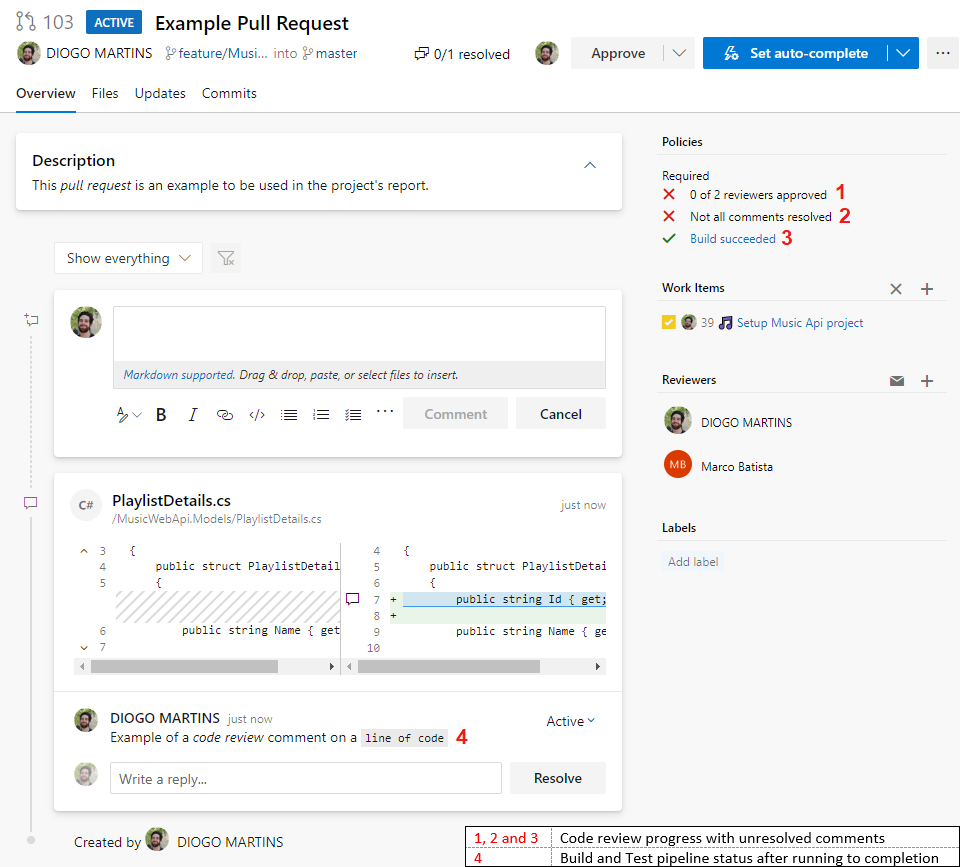
\includegraphics[width=0.75\textwidth]{./Chapter4/Figures/PullRequestExample.png}
	\caption{An example of a pull request in the development repositories}
	\label{fig:PullRequestExample}
\end{figure}

\newpage

\section{Other tools}
The group is also using Microsoft Visual Studio as it's main programming IDE as it's really flexible and it's integration with Nuget, Xamarin and UWP is seamless to the group and offers (almost) no problems and Jetbrains DataGrip as the main database IDE (although sometimes the group also uses pgAdmin for more low level operations on the PostgreSQL database).



\section{Architecture}

Figure~\ref{fig:SystemArchitecture} illustrates the system architecture.

\begin{figure}[!ht]
	\centering
	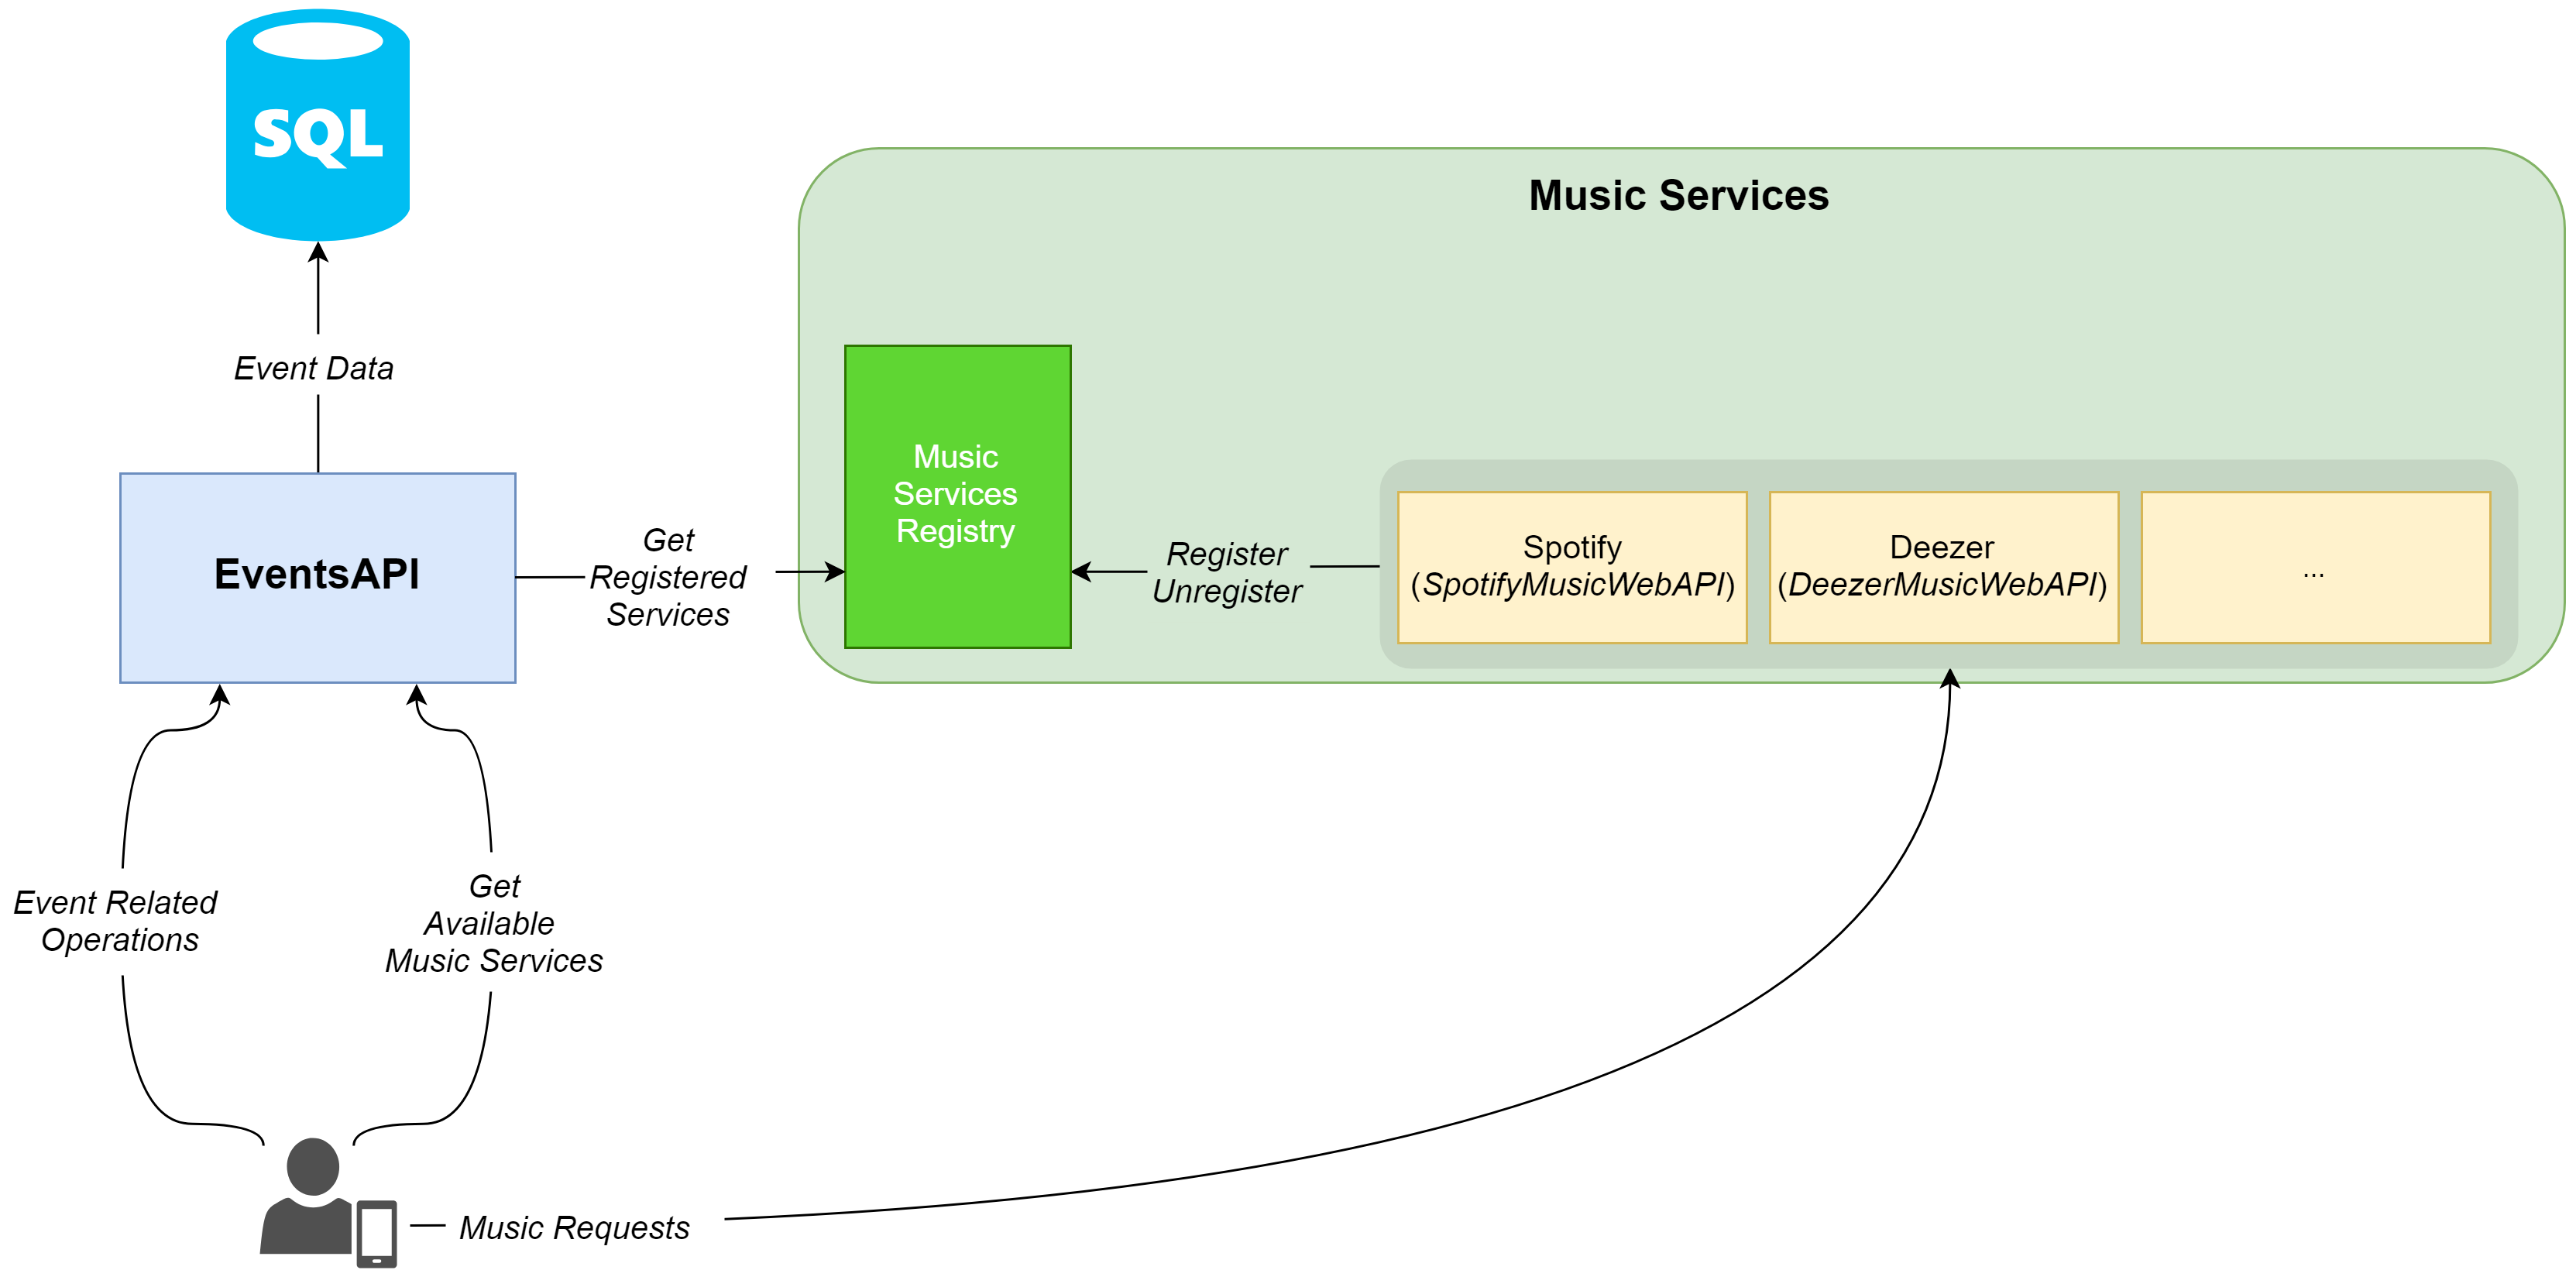
\includegraphics[width=0.75\textwidth]{./Chapter4/Figures/Architecture.png}
	\caption{System architecture.}
	\label{fig:SystemArchitecture}
\end{figure}

\subsection{Client}

The client component of this project is implemented as a mobile application, using the \textit{Android} and \textit{Windows} platform.

\subsection{Server}

The server component is implemented as a REST API, using .NET Core MVC.
\begin{itemize}	
	\item Event API - Supports the event creation and all of its operations (adding, editing and removing guests, expenses, tasks, among others);
	
	\item Music API - Supports the \textit{playlist} creation;
	
	\item Payments API (optional) - Supports the payment of the event's expenses.
	
\end{itemize}

The database operations are supported by the PostgreSQL database engine.

\subsubsection{Observations}

The motivation behind choosing this server-client architecture is the possibility of eventually creating other clients, without having to change the servers that support it.

The reason why the Payments and Media API aren't unified into the Event API is for the sake of having the benefit of the client only communicating with these APIs, yet having the possibility of comunicating with a wide range of services without having to implement them specifically.

The motivation behind the usage of SQL instead of NoSQL database types is because the entities used in this application are of relational types. Also, the atomicty and transactional behaviour that SQL databases support is of importance for consistency across event information.

